\documentclass[border=4pt]{standalone}
% Preámbulo común de las figuras. Cada figura es un documento standalone
% que se compila a SVG con scripts/build_figures.sh
\usepackage[utf8]{inputenc}
\usepackage{amsmath}
\usepackage{tikz}
\usepackage[american, siunitx]{circuitikz}
\usetikzlibrary{arrows.meta,calc,decorations.pathmorphing,patterns}
\tikzset{
  >={Stealth[length=2.2mm]},
  eje/.style={->, thin},
  hilo/.style={thick},
}
% Paleta común: tonos medios legibles sobre fondo claro
\definecolor{azul}{RGB}{31,94,168}
\definecolor{rojo}{RGB}{192,57,43}
\definecolor{verde}{RGB}{39,128,73}
\definecolor{naranja}{RGB}{211,120,30}
\definecolor{morado}{RGB}{125,60,152}

\begin{document}
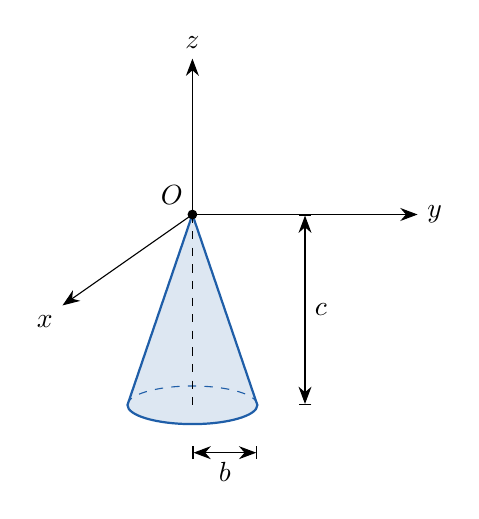
\begin{tikzpicture}[scale=1.1]
  \draw[eje] (0,0) -- (2.6,0) node[right]{$y$};
  \draw[eje] (0,0) -- (0,1.8) node[above]{$z$};
  \draw[eje] (0,0) -- (-1.5,-1.05) node[below left]{$x$};
  \filldraw[draw=azul, fill=azul!15, thick] (0,0) -- (-0.75,-2.2) arc[start angle=180, end angle=360, x radius=0.75, y radius=0.22] -- cycle;
  \draw[azul, dashed] (-0.75,-2.2) arc[start angle=180, end angle=0, x radius=0.75, y radius=0.22];
  \fill (0,0) circle (1.6pt) node[above left]{$O$};
  \draw[dashed] (0,0) -- (0,-2.2);
  \draw[|<->|] (1.3,0) -- node[right]{$c$} (1.3,-2.2);
  \draw[|<->|] (0,-2.75) -- node[below]{$b$} (0.75,-2.75);
\end{tikzpicture}
\end{document}
